\subsection{Liste des matchs}
\vspace{1cm}

L’interface principale devait intégrer la liste des matchs complets à venir pour le reste de la saison. Elle devait également permettre le tri de ces matchs en fonction des différentes poules possibles sans recharger la page.\\

J’ai mis en place un composant sous forme de classe permettant de gérer ces deux différents scénarios, et de renvoyer au choix le tableau de tous les matchs à venir ou le tableau des matchs à venir d’une poule.
Pour fonctionner, cette classe prend en paramètre l’ID d’une poule et renvoi alors le tableau html composé de tous les matchs à venir associés, récupérés depuis la base de données. 
Ce paramètre peut être nul et renvoi dans ce cas la liste complète des matchs à venir sans distinction de poules.

\begin{figure}[!h]
    \centering
    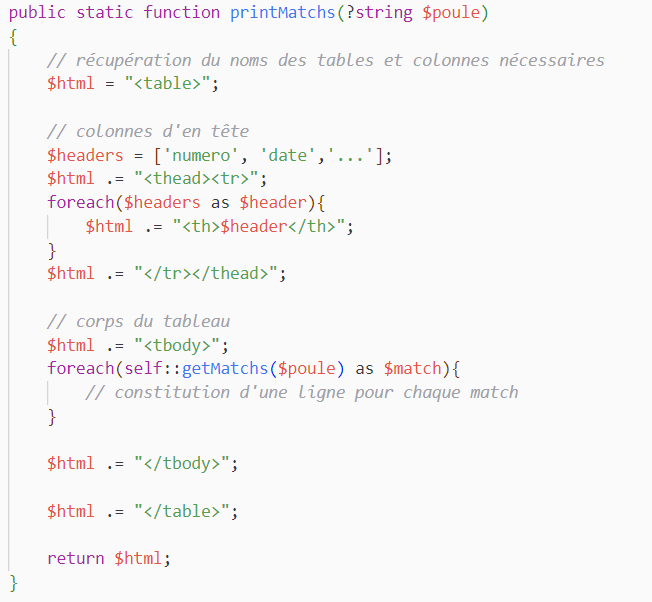
\includegraphics{table}
    \caption{Méthode de construction de tableau pour une poule}
\end{figure}

\newpage

De cette façon, je n’avais qu’à attacher un évènement au changement du SELECT affichant les poules, qui enverrait via AJAX la valeur de celle-ci à une page annexe. Cette page n’aurait alors qu’à renvoyer le bon tableau grâce à cette méthode.

\begin{commentaire}
AJAX (Asynchronous Javascript and XML) est une méthode permettant de faire des requêtes à un serveur web de façon asynchrone, et de récupérer la réponse de celui-ci sans recharger la page.
\end{commentaire}

Pour faciliter l’envoi et la gestion de ces requêtes, j’ai utilisé la bibliothèque JQuery déjà très largement utilisée dans le cadre de cette transition numérique.

\begin{figure}[!h]
    \centering
    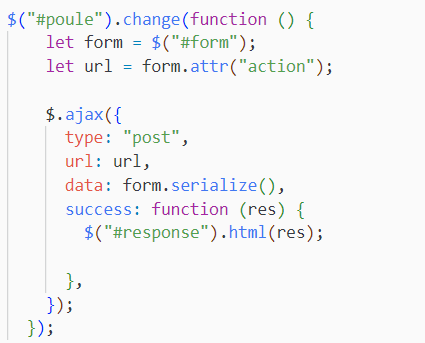
\includegraphics{ajax}
    \caption{Fonction AJAX au changement d'une poule}
\end{figure}

